% lint-skip: 未完成ステータス（figure/table caption 未対応，人手チェック時に解消予定）
\documentclass[../../main.tex]{subfiles}
\begin{document}

\begin{flushright}
  \footnotesize\textit{【自動文字起こし・要確認】}
\end{flushright}

{\bf [解答]} $\angle A_n O B_n = \theta_n$ とおくと，題意から
帰納的に
\[ \theta_n = \left(\dfrac{1}{2}\right)^{n-1} \theta \cdots \text{①} \]
右下図で，
\[ OA_n = a_n \]
\[ OB_{n+1} = a_{n+1} \]
だから
\[
  \begin{cases} a_n \cos\left(\left(\dfrac{1}{2}\right)^n \theta\right) = a_{n+1} \\ a_1 = 1
\end{cases} \]
となり，
\[ a_n = \cos\left\{ \left(\dfrac{1}{2}\right)^{n-1} \theta \right\} \cdots \cos\dfrac{\theta}{8} \cos\dfrac{\theta}{4} \cos\dfrac{\theta}{2} \]
である

\paragraph{(1)}
\[ a_3 \cdot \sin\dfrac{\theta}{4} = \sin\dfrac{\theta}{4} \cdot \cos\dfrac{\theta}{4} \cdot \cos\dfrac{\theta}{2} = \dfrac{1}{2} \sin\dfrac{\theta}{2} \cdot \cos\dfrac{\theta}{2} = \dfrac{1}{4} \sin\theta \quad \text{//} \]

\paragraph{(2)}

$a_n \sin\dfrac{\theta}{2^{n-1}} = A_n$ も，(1)と同じように計算して
\[ A_n = \left(\dfrac{1}{2}\right)^{n-1} \sin\theta \]
だから
\[ a_n = \dfrac{ \left(\dfrac{1}{2}\right)^{n-1} \theta }{ \sin\left\{ \left(\dfrac{1}{2}\right)^{n-1} \theta \right\} } \cdot \dfrac{\sin\theta}{\theta} \to \dfrac{\sin\theta}{\theta} \quad (n \to \infty) \quad \text{//} \]

\begin{figure}[htbp]
  \centering
  \begin{minipage}{0.52\linewidth}
    \centering
    % 図示用に O=(0,3), A_1=(-3,0), B_1=(3,0) を選ぶ。
    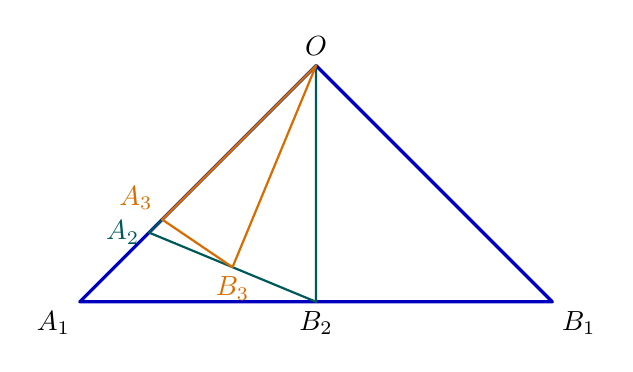
\begin{tikzpicture}[scale=1.0,line join=round]
      \coordinate (O) at (0,3);
      \coordinate (Aone) at (-3,0);
      \coordinate (Bone) at (3,0);
      \coordinate (Btwo) at (0,0);
      \coordinate (Atwo) at (-2.121,0.879);
      \coordinate (Bthree) at (-1.061,0.4395);
      \coordinate (Athree) at (-1.954,1.045);
      \draw[blue!75!black,very thick] (O)--(Aone)--(Bone)--cycle;
      \draw[gray!60,dashed] (O)--(Btwo);
      \draw[teal!70!black,thick] (O)--(Atwo)--(Btwo)--cycle;
      \draw[orange!85!black,thick] (O)--(Athree)--(Bthree)--cycle;
      \node[above] at (O) {$O$};
      \node[below left] at (Aone) {$A_1$};
      \node[below right] at (Bone) {$B_1$};
      \node[below] at (Btwo) {$B_2$};
      \node[left,teal!70!black] at (Atwo) {$A_2$};
      \node[above left,orange!85!black] at (Athree) {$A_3$};
      \node[below,orange!85!black] at (Bthree) {$B_3$};
    \end{tikzpicture}
    \par\smallskip $n=1,2,3$ の構成
  \end{minipage}\hfill
  \begin{minipage}{0.42\linewidth}
    \centering
    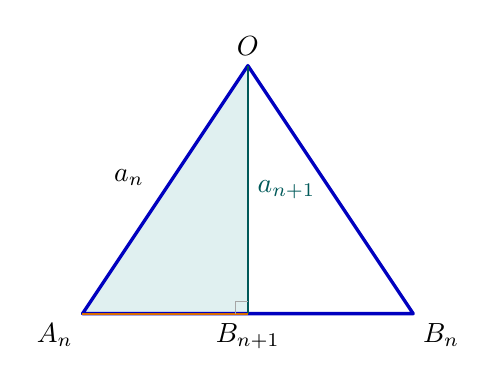
\begin{tikzpicture}[scale=1.05,line join=round]
      \coordinate (O) at (0,3);
      \coordinate (An) at (-2,0);
      \coordinate (Bn) at (2,0);
      \coordinate (Bnext) at (0,0);
      \fill[teal!12] (O)--(An)--(Bnext)--cycle;
      \draw[blue!75!black,very thick] (O)--(An)--(Bn)--cycle;
      \draw[teal!70!black,thick] (O)--(Bnext);
      \draw[orange!85!black,thick] (An)--(Bnext);
      \draw[gray!70] (-0.15,0)--(-0.15,0.15)--(0,0.15);
      \node[above] at (O) {$O$};
      \node[below left] at (An) {$A_n$};
      \node[below right] at (Bn) {$B_n$};
      \node[below] at (Bnext) {$B_{n+1}$};
      \node[left] at (-1.14,1.65) {$a_n$};
      \node[right,teal!70!black] at (0,1.5) {$a_{n+1}$};
    \end{tikzpicture}
    \par\smallskip 一般の $n$ における直角三角形
  \end{minipage}
  \caption{辺の中点を使った二等辺三角形の反復構成}
\end{figure}

\end{document}
